%%%%%%%%%%%%%%%%%%%%%%%%%%%%%%%%%%%%%%%%%
% Beamer Presentation
% LaTeX Template
% Version 2.0 (March 8, 2022)
%
% This template originates from:
% https://www.LaTeXTemplates.com
%
% Author:
% Vel (vel@latextemplates.com)
%
% License:
% CC BY-NC-SA 4.0 (https://creativecommons.org/licenses/by-nc-sa/4.0/)
%
%%%%%%%%%%%%%%%%%%%%%%%%%%%%%%%%%%%%%%%%%

%----------------------------------------------------------------------------------------
%	PACKAGES AND OTHER DOCUMENT CONFIGURATIONS
%----------------------------------------------------------------------------------------

\documentclass[
	11pt, % Set the default font size, options include: 8pt, 9pt, 10pt, 11pt, 12pt, 14pt, 17pt, 20pt
	%t, % Uncomment to vertically align all slide content to the top of the slide, rather than the default centered
	%aspectratio=169, % Uncomment to set the aspect ratio to a 16:9 ratio which matches the aspect ratio of 1080p and 4K screens and projectors
]{beamer}

\graphicspath{{images/}{./}} % Specifies where to look for included images (trailing slash required)

\usepackage{booktabs} % Allows the use of \toprule, \midrule and \bottomrule for better rules in tables
\usepackage{animate}
\usepackage{quoting}

\usepackage{algorithm} 
\usepackage{algpseudocode}
\usepackage{multirow}
\usepackage{wrapfig}
\usepackage{animate,media9,movie15}

%----------------------------------------------------------------------------------------
%	SELECT LAYOUT THEME
%----------------------------------------------------------------------------------------

% Beamer comes with a number of default layout themes which change the colors and layouts of slides. Below is a list of all themes available, uncomment each in turn to see what they look like.

%\usetheme{default}
%\usetheme{AnnArbor}
%\usetheme{Antibes}
%\usetheme{Bergen}
%\usetheme{Berkeley}
%\usetheme{Berlin}
%\usetheme{Boadilla}
%\usetheme{CambridgeUS}
%\usetheme{Copenhagen}
%\usetheme{Darmstadt}
%\usetheme{Dresden}
%\usetheme{Frankfurt}
%\usetheme{Goettingen}
%\usetheme{Hannover}
%\usetheme{Ilmenau}
%\usetheme{JuanLesPins}
%\usetheme{Luebeck}
%\usetheme{Madrid}
%\usetheme{Malmoe}
%\usetheme{Marburg}
%\usetheme{Montpellier}
\usetheme{PaloAlto}
%\usetheme{Pittsburgh}
%\usetheme{Rochester}
%\usetheme{Singapore}
%\usetheme{Szeged}
%\usetheme{Warsaw}
\usepackage{ragged2e}
\usepackage{microtype}
\usepackage{xcolor}
\definecolor{verde}{RGB}{40,167,69}
\definecolor{branco}{RGB}{255,255,255}

%\setbeamercolor{frametitle}{bg=verde, fg=branco}
%\setbeamercolor{sidebar}{bg=verde, fg=branco}
%\setbeamercolor*{structure}{bg=branco}

%----------------------------------------------------------------------------------------
%	SELECT COLOR THEME
%----------------------------------------------------------------------------------------

% Beamer comes with a number of color themes that can be applied to any layout theme to change its colors. Uncomment each of these in turn to see how they change the colors of your selected layout theme.

%\usecolortheme{albatross}
%\usecolortheme{beaver}
%\usecolortheme{beetle}
%\usecolortheme{crane}
%\usecolortheme{dolphin}
%\usecolortheme{dove}
%\usecolortheme{fly}
%\usecolortheme{lily}
%\usecolortheme{monarca}
%\usecolortheme{seagull}
%\usecolortheme{seahorse}
%\usecolortheme{spruce}
\usecolortheme{whale}
%\usecolortheme{wolverine}

%---------------------------------------------------------------------------------------
%	SELECT FONT THEME & FONTS-
%----------------------------------------------------------------------------------------

% Beamer comes with several font themes to easily change the fonts used in various parts of the presentation. Review the comments beside each one to decide if you would like to use it. Note that additional options can be specified for several of these font themes, consult the beamer documentation for more information.

\usefonttheme{default} % Typeset using the default sans serif font
%\usefonttheme{serif} % Typeset using the default serif font (make sure a sans font isn't being set as the default font if you use this option!)
%\usefonttheme{structurebold} % Typeset important structure text (titles, headlines, footlines, sidebar, etc) in bold
%\usefonttheme{structureitalicserif} % Typeset important structure text (titles, headlines, footlines, sidebar, etc) in italic serif
%\usefonttheme{structuresmallcapsserif} % Typeset important structure text (titles, headlines, footlines, sidebar, etc) in small caps serif

%------------------------------------------------

%\usepackage{mathptmx} % Use the Times font for serif text
\usepackage{palatino} % Use the Palatino font for serif text

%\usepackage{helvet} % Use the Helvetica font for sans serif text
\usepackage[default]{opensans} % Use the Open Sans font for sans serif text
%\usepackage[default]{FiraSans} % Use the Fira Sans font for sans serif text
%\usepackage[default]{lato} % Use the Lato font for sans serif text

%----------------------------------------------------------------------------------------
%	SELECT INNER THEME
%----------------------------------------------------------------------------------------

% Inner themes change the styling of internal slide elements, for example: bullet points, blocks, bibliography entries, title pages, theorems, etc. Uncomment each theme in turn to see what changes it makes to your presentation.

%\useinnertheme{default}
\useinnertheme{circles}
%\useinnertheme{rectangles}
%\useinnertheme{rounded}
%\useinnertheme{inmargin}

%----------------------------------------------------------------------------------------
%	SELECT OUTER THEME
%----------------------------------------------------------------------------------------

% Outer themes change the overall layout of slides, such as: header and footer lines, sidebars and slide titles. Uncomment each theme in turn to see what changes it makes to your presentation.

%\useoutertheme{default}
%\useoutertheme{infolines}
%\useoutertheme{miniframes}
%\useoutertheme{smoothbars}
%\useoutertheme{sidebar}
%\useoutertheme{split}
%\useoutertheme{shadow}
%\useoutertheme{tree}
%\useoutertheme{smoothtree}

%\settemplate{footline} % Uncomment this line to remove the footer line in all slides
%\setbeamertemplate{footline}[page number] % Uncomment this line to replace the footer line in all slides with a simple slide count

%\setbeamertemplate{navigation symbols}{} % Uncomment this line to remove the navigation symbols from the bottom of all slides

\makeatletter
\logo{
\includegraphics[width=0.123\linewidth]{logo.png}}
\makeatother

%----------------------------------------------------------------------------------------
%	PRESENTATION INFORMATION
%----------------------------------------------------------------------------------------

\title[Quick Sort]{Método de Ordenação | QuickSort} % The short title in the optional parameter appears at the bottom of every slide, the full title in the main parameter is only on the title page

\subtitle{Código e Análise de Complexidade} % Presentation subtitle, remove this command if a subtitle isn't required

\author[]{Larissa; Mauricio Monteiro; Paulo Henrique} % Presenter name(s), the optional parameter can contain a shortened version to appear on the bottom of every slide, while the main parameter will appear on the title slide

\institute[UFMG]{ UFMG | ICEx \\ Departamento de Ciência da Computação | DCC \\ Ambientes de Computação } % Your institution, the optional parameter can be used for the institution shorthand and will appear on the bottom of every slide after author names, while the required parameter is used on the title slide and can include your email address or additional information on separate lines

\date[\today]{} 
% Presentation date or conference/meeting name, the optional parameter can contain a shortened version to appear on the bottom of every slide, while the required parameter value is output to the title slide

%----------------------------------------------------------------------------------------

\begin{document}

%----------------------------------------------------------------------------------------
%	TITLE SLIDE
%----------------------------------------------------------------------------------------

\begin{frame}
	\titlepage % Output the title slide, automatically created using the text entered in the PRESENTATION INFORMATION block above
\end{frame}

%----------------------------------------------------------------------------------------
%	TABLE OF CONTENTS SLIDE
%----------------------------------------------------------------------------------------

% The table of contents outputs the sections and subsections that appear in your presentation, specified with the standard \section and \subsection commands. You may either display all sections and subsections on one slide with \tableofcontents, or display each section at a time on subsequent slides with \tableofcontents[pausesections]. The latter is useful if you want to step through each section and mention what you will discuss.

\begin{frame}
	\frametitle{Visão geral da apresentação} % Slide title, remove this command for no title
	
	\tableofcontents % Output the table of contents (all sections on one slide)
	%\tableofcontents[pausesections] % Output the table of contents (break sections up across separate slides)
\end{frame}

%----------------------------------------------------------------------------------------
%	PRESENTATION BODY SLIDES
%----------------------------------------------------------------------------------------
\section{Introdução} 
\begin{frame}
	\frametitle{Introdução}
	\justifying O trabalho tem como objetivo:
	\bigskip
	\bigskip
	{\small
	\begin{itemize}
		\item \justifying traduzir o código escrito na \textit{linguagem C} para a \textit{linguagem Python};
		\item \justifying compreender o funcionamento do algoritmo proposto;
		\item \justifying explicar a \textbf{Análise de Complexidade} do código.
	\end{itemize}
	}
\end{frame}

\begin{frame}
	\frametitle{Código em C}
	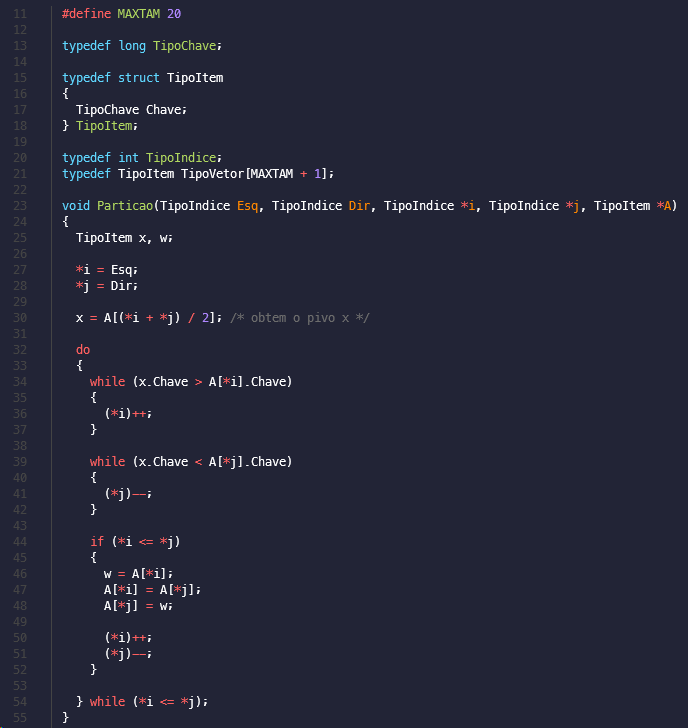
\includegraphics[width=0.7\linewidth]{quick_sort_in_c_particao}
\end{frame}
\begin{frame}
	\frametitle{Código em C}
	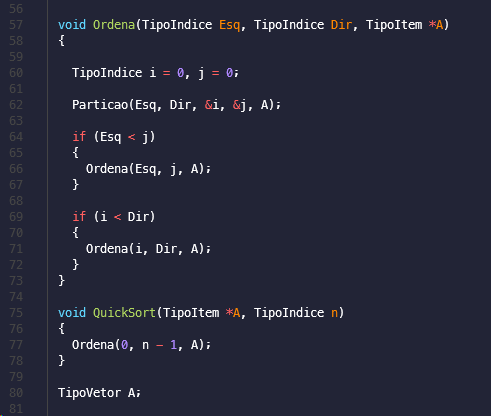
\includegraphics[width=0.7\linewidth]{quick_sort_in_c_ordena}
\end{frame}

\section{História e surgimento}
\begin{frame}
	\frametitle{História e surgimento}
	\justifying Ao analisar o funcionamento do, descobrimos que o algoritmo é um método de ordenação muito conhecido chamada \textbf{QuickSort}.
	
	\bigskip
	
	\small
	Quicksort é o algoritmo de ordenação interna mais rápido que se conhece para uma ampla variedade de situações, sendo provavelmente mais utilizado do que qualquer outro algoritmo.
	
	\bigskip
	\begin{wrapfigure}{l}{0.18\textwidth}
		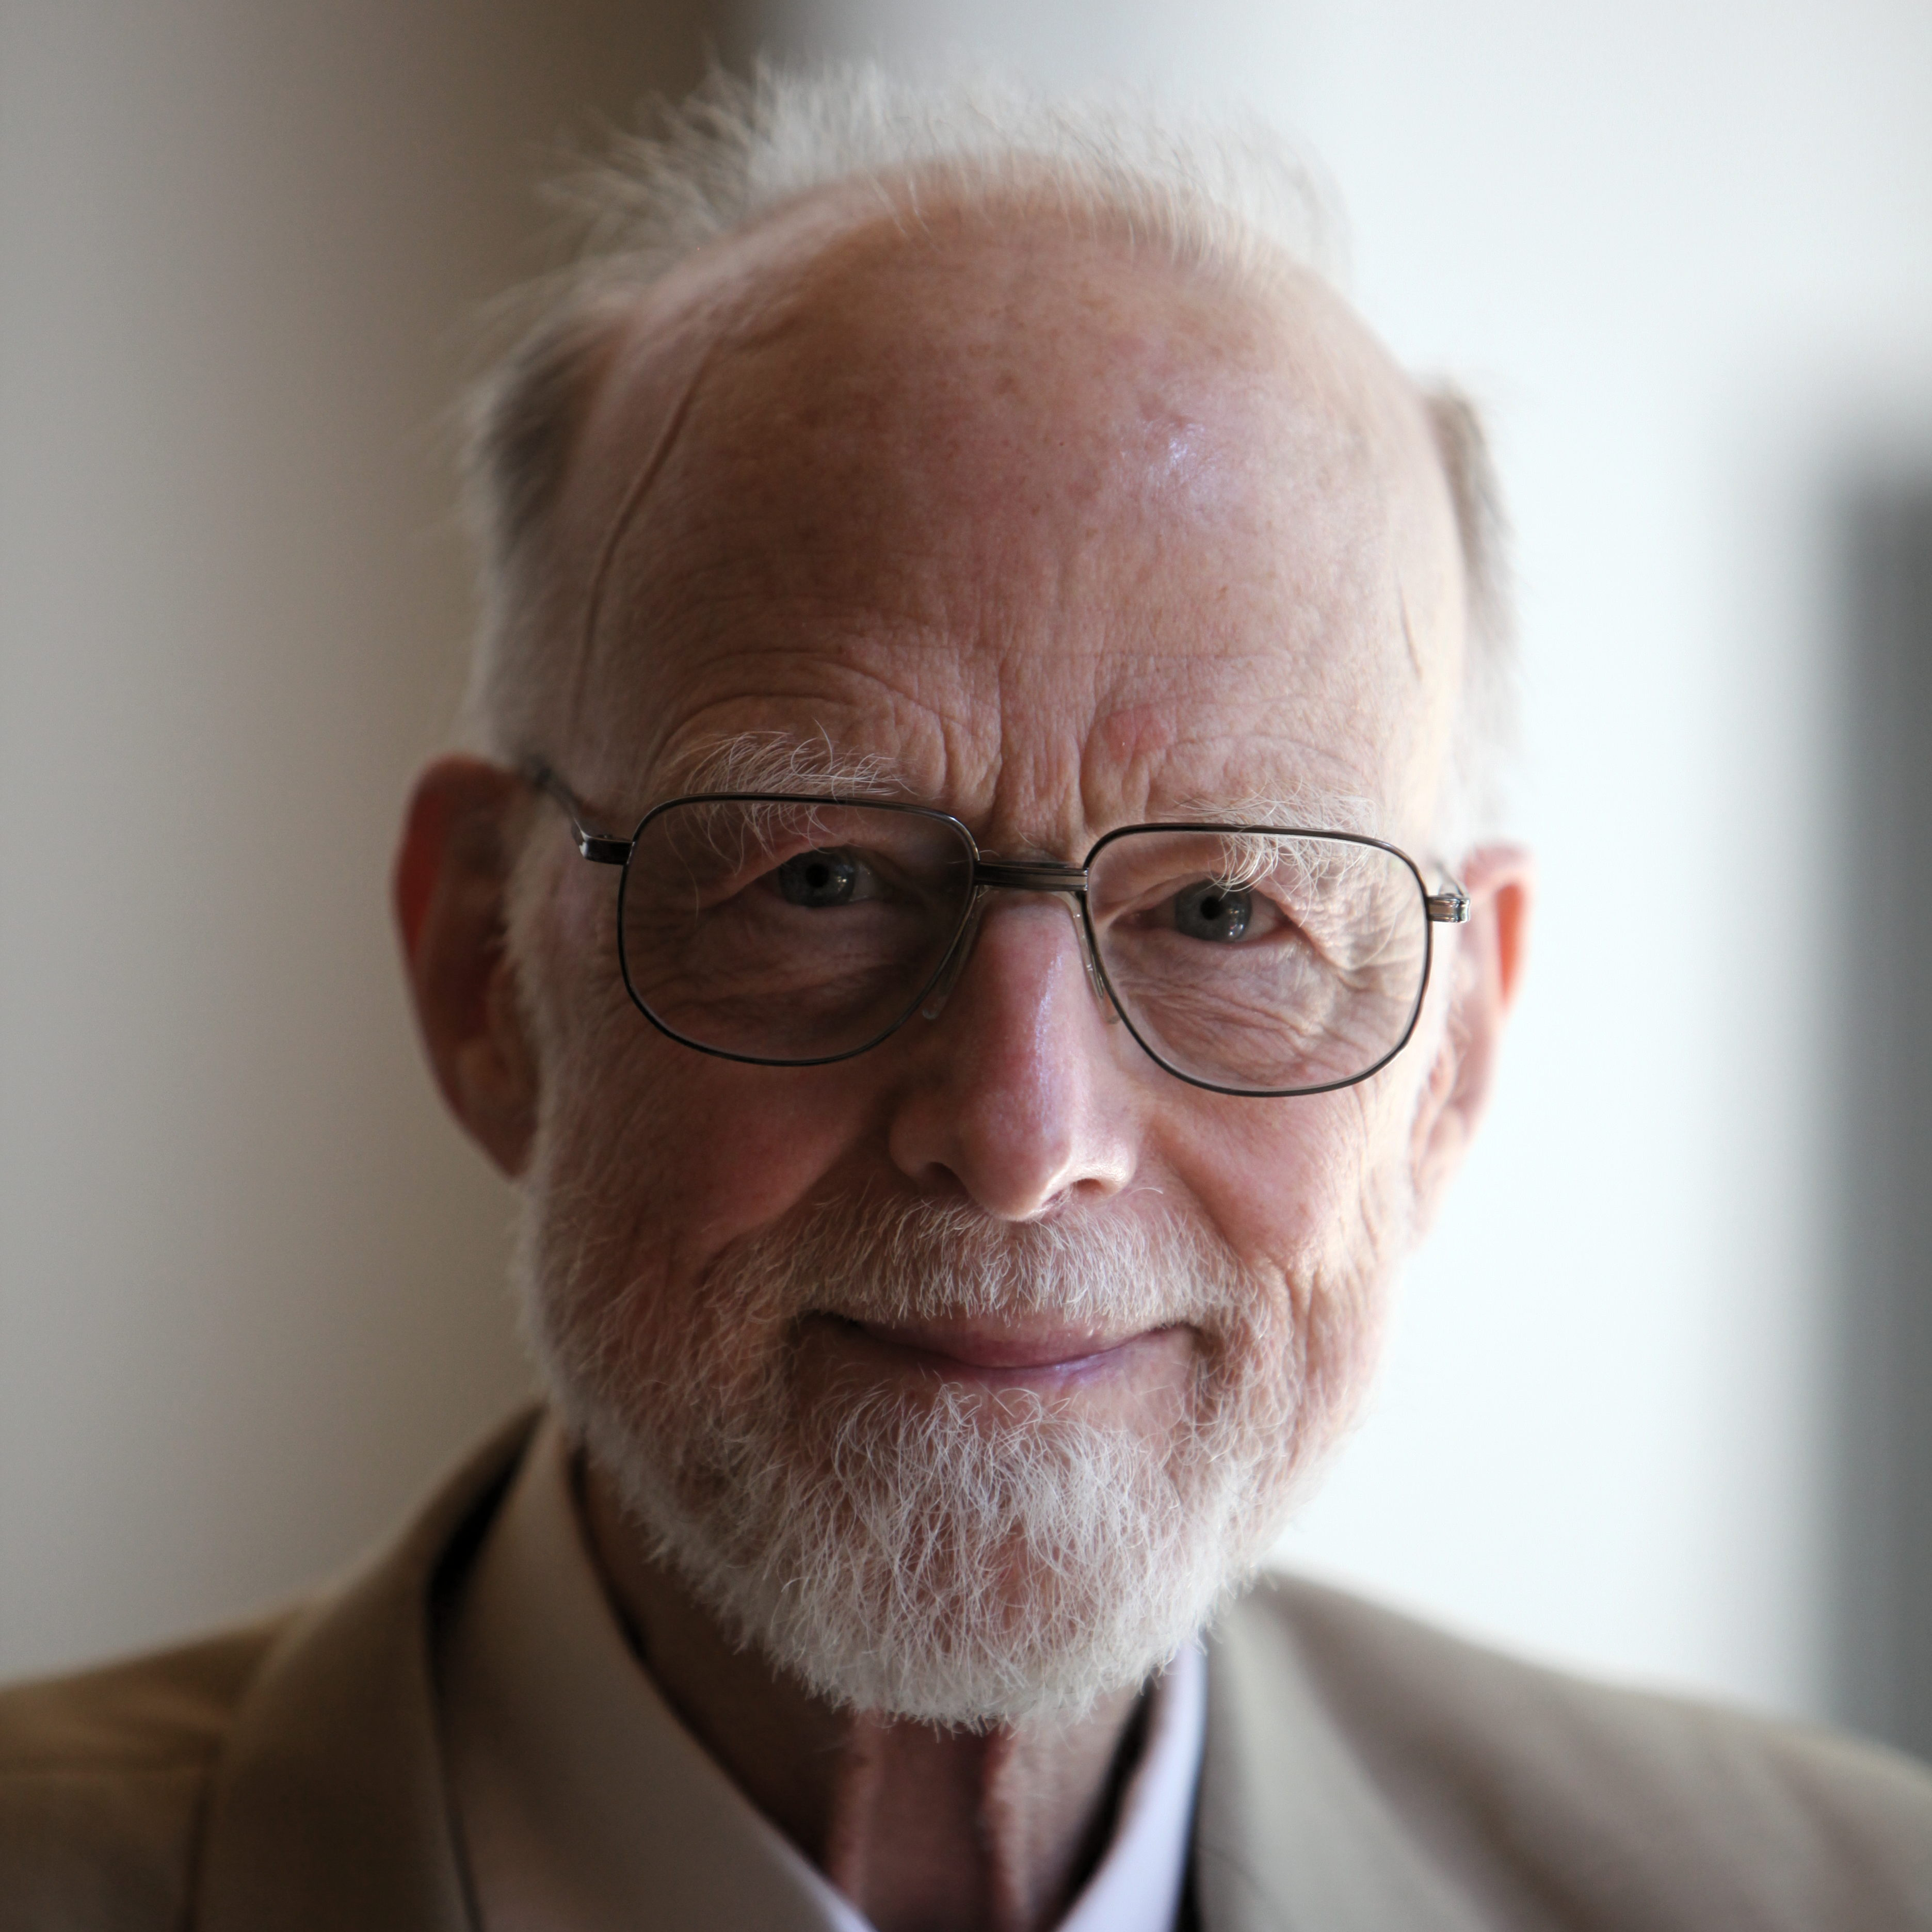
\includegraphics[width=1\linewidth]{Sir_Tony_Hoare_IMG_5125.jpg}
	\end{wrapfigure}

	O algoritmo foi inventado por \textbf{Charles Antony Richard Hoare} em 1960, quando visitava a Universidade de Moscou como estudante.
	
	\bigskip
	O algoritmo foi publicado mais tarde por Hoare (1962), após uma série de refinamentos.
	

\end{frame}

\section{Código em Python}
\begin{frame}
	\frametitle{Código em Python}
	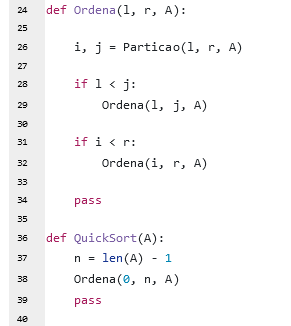
\includegraphics[width=0.6\linewidth]{quick_sort_in_python_ordena}
\end{frame}

\begin{frame}
	\frametitle{Código em Python}
	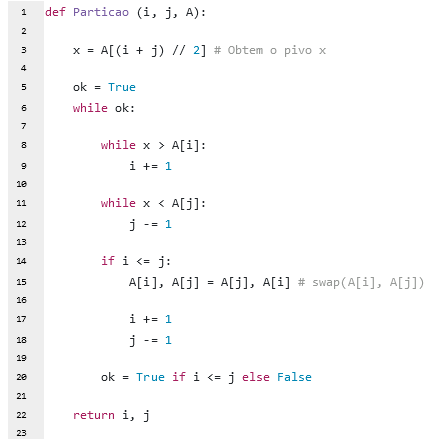
\includegraphics[width=0.7\linewidth]{quick_sort_in_python_particao}
\end{frame}

\section{Lógica do Algoritmo}
\begin{frame}
	\frametitle{Lógica do Algoritmo}
	
	{\tiny
	\begin{wrapfigure}{r}{0.5\textwidth}
		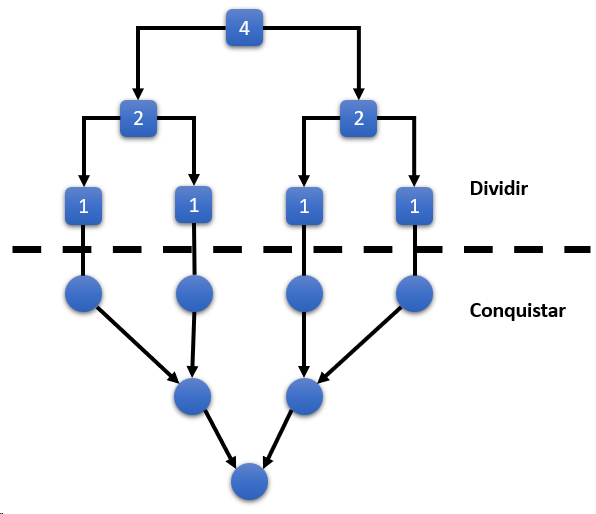
\includegraphics[width=1\linewidth]{dividir_conquistar}
	\end{wrapfigure}

	\justifying O QuickSort utiliza de um método para a construção de algoritmos conhecido como \textbf{a estratégia de divisão e conquista}. A estratégia consiste em dividir um problema maior recursivamente em problemas menores até que o problema possa ser resolvido diretamente
	
	\bigskip
	
	\begin{itemize}		
		\item \justifying A idéia básica é a de partir o problema de ordenar um conjunto $A = \{a_0, a_1, \cdots, a_{n-1}, a_{n} \}$ com $n$ itens em \textbf{dois problemas menores}.
		
		\bigskip
		
		\item \justifying Os problemas menores são ordenados independentemente e depois os resultados são combinados para produzir a solução do problema maior.
	\end{itemize}
	}
\end{frame}

\begin{frame}
	\frametitle{Lógica do Algoritmo}
	\justifying
	\begin{itemize}
		\item \justifying A parte mais delicada deste método é relativa ao procedimento partição, o qual tem que rearranjar o vetor $A = \{ a_{\text{esq}},\cdots, a_{\text{dir}} \}$ através da escolha arbitrária de um item $x$ do vetor chamado \textbf{pivô}.
		
		\bigskip
		
		\item \justifying Ao final o vetor $A$ estará particionado em uma \textbf{parte esquerda} com chaves \textbf{menores ou iguais} a $x$ e uma \textbf{parte direita} com chaves \textbf{maiores ou iguais} a $x$.
	\end{itemize}
\end{frame}

\begin{frame}
	\frametitle{Lógica do Algoritmo}
	\justifying
	{\small Este comportamento pode ser descrito pelo seguinte algoritmo:}
	\begin{enumerate}
		\item \justifying {\tiny escolha arbitrariamente um item do vetor e o coloque em $x$;}
		\item \justifying {\tiny percorra o vetor a partir da esquerda até que um item $a_{i} > x$ é encontrado.}
		\item \justifying {\tiny da mesma forma percorra o vetor a partir da direita até que um item $a_{j} \le x$ é encontrado;}
		\item \justifying {\tiny como os dois itens $A_{i}$ e $A_{j}$ estão fora de lugar no vetor final então \textbf{troque-os de lugar};}
		\item \justifying {\tiny continue este processo até que os apontamentos $i$ e $j$ se \textbf{cruzem} em algum pronto do vetor.}
	\end{enumerate}
	
\end{frame}

\begin{frame}
	\frametitle{Lógica do Algoritmo}
	\justifying
	Ao final o vetor $A = \{ a_{\text{esq}},\cdots, a_{\text{dir}} \}$ está parcionado de tal forma que:
	
	\begin{itemize}
		\item \justifying {\small os itens em $a_{\text{esq}}, a_{\text{esq} + 1}, \cdots, a_{j}$ são \textbf{menores} ou iguais a $x$},
		\item \justifying {\small os itens em $a_{i}, a_{i+1}, \cdots, a_{dir}$ são \textbf{maiores} ou iguais a $x$}.
	\end{itemize}

\end{frame}

\section{Passo a Passo} 
\begin{frame}
	\frametitle{Passo a Passo}
	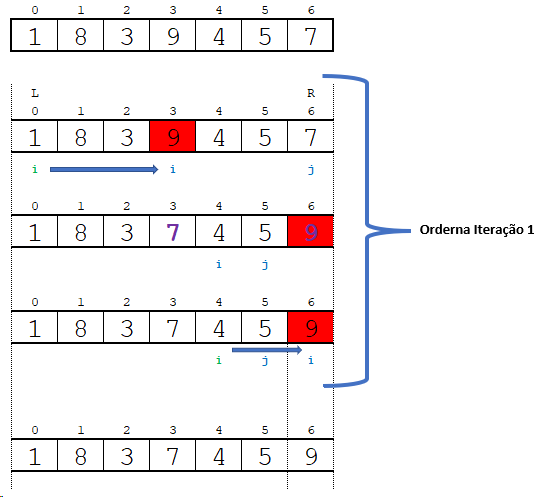
\includegraphics[width=0.8\linewidth]{o1}
\end{frame}
\begin{frame}
	\frametitle{Passo a Passo}
	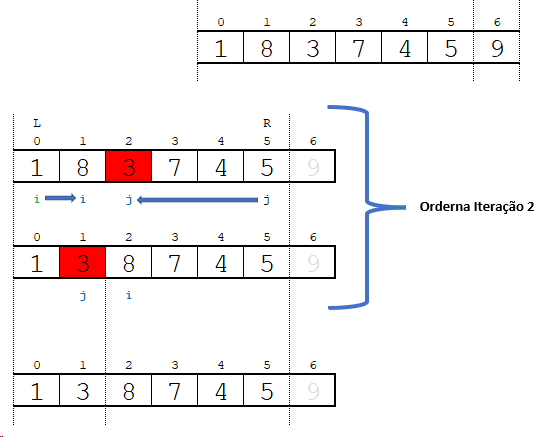
\includegraphics[width=0.8\linewidth]{o2}
\end{frame}
\begin{frame}
	\frametitle{Passo a Passo}
	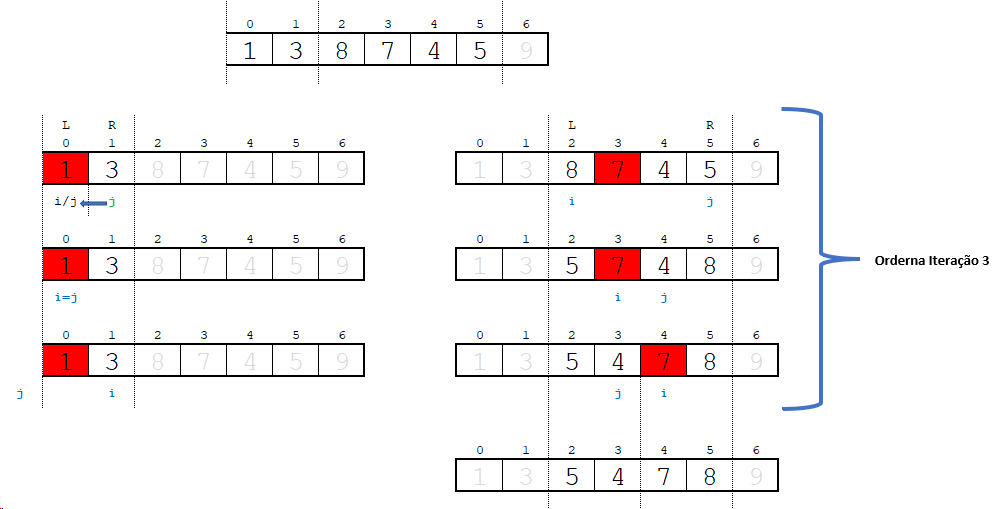
\includegraphics[width=0.8\linewidth]{o3}
\end{frame}
\begin{frame}
	\frametitle{Passo a Passo}
	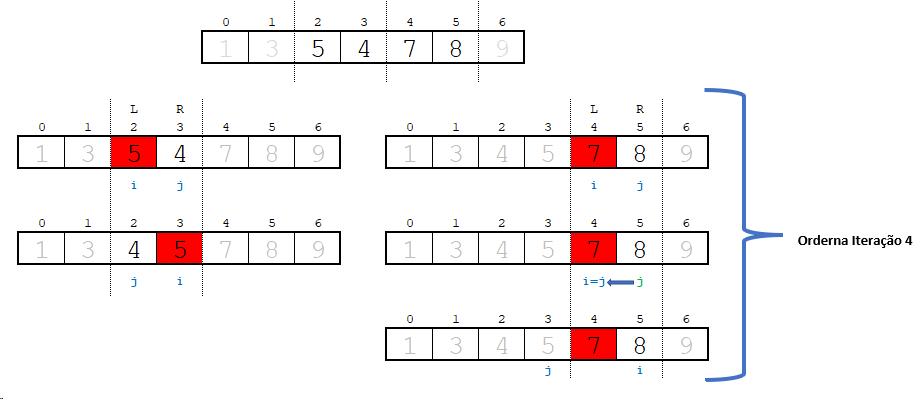
\includegraphics[width=0.9\linewidth]{o4}
\end{frame}
\begin{frame}
	\frametitle{Animações}
	\justifying
	
	Animação do exemplo proposto:
	
	\begin{center}
	\animategraphics[loop,width=10cm]{0.5}{an-}{0}{47}
	\end{center}

	Outra animação de exemplo:
	\begin{center}
		\animategraphics[loop,width=5cm]{1.1}{anim-}{0}{69}
	\end{center}

\end{frame}

\begin{frame}
	\frametitle{Vídeo}
	\justifying
	
	\textbf{Vídeo:} Quick Sort with Hungarian, folk dance:
	
\begin{figure}
	\movie[width=10cm,height=6cm,poster]{}{video.mp4}
	%    \animategraphics[controls,autoplay,loop,scale=0.5]{10}{Wildlife}{}{}
	%    \includemovie[autoplay]{Wildlife.wmv}
	
	%\includemovie[poster,autoplay,externalviewer,inline=false,text={\small(Quick Sort with Hungarian, folk dance)}]{10cm}{6cm}{video.mp4}
	
	%    \flashmovie{Wildlife.wmv}
\end{figure}
	
\end{frame}

\section{Análise de Complexidade} 
\begin{frame}
	\frametitle{Análise de Complexidade | Pior Caso}
	{\tiny \justifying
	O Quicksort é ineficiente para conjuntos de dados já \underline{ordenados de maneira crescente e decrescente} e também se \underline{todos os elementos} do conjunto \underline{forem iguais}, pois a escolha do pivô se torna inadequada.}
	
	\begin{center}
		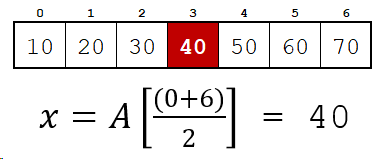
\includegraphics[width=0.5\linewidth]{exemplo1}
	\end{center}
	{\tiny
	\begin{itemize}
		\item \justifying No exemplo acima escolha sistemática dos extremos de um conjuntos de dados já ordenado leva ao seu \textbf{pior caso}.
	
		\item \justifying As partições serão extremamente \textbf{desiguais}, e o procedimento $Ordena(...)$ será chamado recursivamente $n$ vezes, \textbf{eliminando apenas um item} em cada chamada.
		
		\item \justifying Esta situação é desastrosa pois o número de comparações chegar ser $\frac{n^{2}}{2}$, e o tamanho da pilha necessária para as chamadas recursivas chega ser de tamanho $n$.
	\end{itemize}
	}

	\begin{center}
		Sendo a \textbf{classe de complexidade} do \textbf{pior caso} igual a $O(n^{2})$.
	\end{center}
\end{frame}

\begin{frame}
	\frametitle{Análise de Complexidade | Melhor Caso}
	
	{\small
	\begin{itemize}
		\item A melhor situação possível ocorre quando cada partição divide o arquivo em duas partes iguais.
		\item Sendo sua função de complexidade:
		
		\begin{center}
			$C(n) = 2*C\bigg(\frac{n}{2}\bigg) + n - 1$
		\end{center}
		
		\item Onde $C\bigg(\frac{n}{2}\bigg)$ representa o custo de ordenar uma das metades e $n$ é o custo de examinar cada item.
	\end{itemize}
	}
\end{frame}

\begin{frame}
	\frametitle{Análise de Complexidade | Caso Médio}
	
	{\small
		\begin{itemize}
			\item A solução para esta recorrência é $C(n) = n*\log(n) - n + 1$.
			\item Segundo \textbf{Sedgewick} e \textbf{Flajolet} (1996, p. 17) o caso médio do número de comparações realizadas são de: 
		
			\begin{center}
			$C(n) \approx 1.386 * n*\log(n) - 0.846*n$
			\end{center}
	
			\item Significa que a \textbf{classe de complexidade} do \textbf{tempo médio} da execução é:
			\begin{center}
			$O\bigg(n*\log(n)\bigg)$.
			\end{center}
		\end{itemize}
	}
\end{frame}

\begin{frame}
	\frametitle{Classificações}
	{\tiny
	\begin{table}[]
		\begin{tabular}{l|l}
			Classe & Algoritmo de ordenação \\
			\\ \hline \\
			Estrutura de Dados & Array, Listas ligadas \\
			\\ \hline \\
			Complexidade do Pior Caso & $O(n^{2})$ \\
			\\ \hline \\
			Complexidade do Caso Médio & $O\bigg(n*\log(n)\bigg)$ \\
			\\ \hline \\
			Complexidade do Melhor Caso & $O\bigg(n*\log(n)\bigg)$ \\
			\\ \hline \\
			Complexidade do Pior Caso de Espaços & $O(n)$ \\ 
			\\ \hline \\
			Estabilidade & \textbf{Não}-Estável
		\end{tabular}
	\end{table}
	}
\end{frame}


%----------------------------------------------------------------------------------------
%	CLOSING SLIDE
%----------------------------------------------------------------------------------------

\begin{frame}[plain] % The optional argument 'plain' hides the headline and footline
	\begin{center}
		
		
\includegraphics[width=0.3\linewidth]{logo.png}
		
		\bigskip
		
		{\Huge Obrigado.}
		
		\bigskip\bigskip % Vertical whitespace
		
		{\LARGE Perguntas?}
	\end{center}
\end{frame}

%----------------------------------------------------------------------------------------

\end{document} 